%!TEX root = ../MasterThesis.tex

\chapter{Concept for a system supporting \gls{E-commerce} fraud investigations} % (fold)
\label{cha:system_concept}

This chapter looks specifically into the concept of a collaborative system that will improve the situation described in the scenario in Section~\ref{sec:scope_thesis}. To do this, the chapter will discuss the overall concept of such a system on an high level without going to much into implementation specific details. At the end, the chapter will have answered the question of what the system is, and what should be able to achieve with it. In addition to these discussions, the chapter will further look into existing design approaches and analyses why they are of no use for the specific scenario of this Master Thesis.

% sub chapter design overview
%!TEX root = ../MasterThesis.tex

\section{Collaboration on \gls{E-commerce} fraud incidents}
\label{sec:concept_overview}

Based on the explanations in Chapter~\ref{cha:context_analysis}, and especially the scope definition for this Master Thesis in Section~\ref{sec:scope_thesis}, the collaborative system for investigating \gls{E-commerce} fraud incidents has to answer the central question:\@

\begin{quotation}
  \textit{Is this transaction really a valid \gls{E-commerce} transaction?}
\end{quotation}

Looking into the stakeholders, who can provide useful information to decide it, one will come up with:\@

\begin{enumerate}
    \item \textbf{Merchants}, who can provide additional information of each \gls{E-commerce} transaction in question.
    \item \textbf{\gls{PSP}s/issuers}, who have information about the credit card usage patterns and the original credit card owners.
    \item \textbf{\gls{LSP}s}, who can offer information about whether an order has already been shipped or not, and in the former case to whom it has been handed over.
\end{enumerate}

Ideally, each of those participants would make parts of their internal databases available for the others to access and query for information in a shared information space. That would allow those stakeholders, who have to authorize or validate a suspicious credit card transaction, to analyse all available information as depicted in the Figure~\ref{fig:images_system_overview}.\@

\begin{figure}[H]
	\centering
		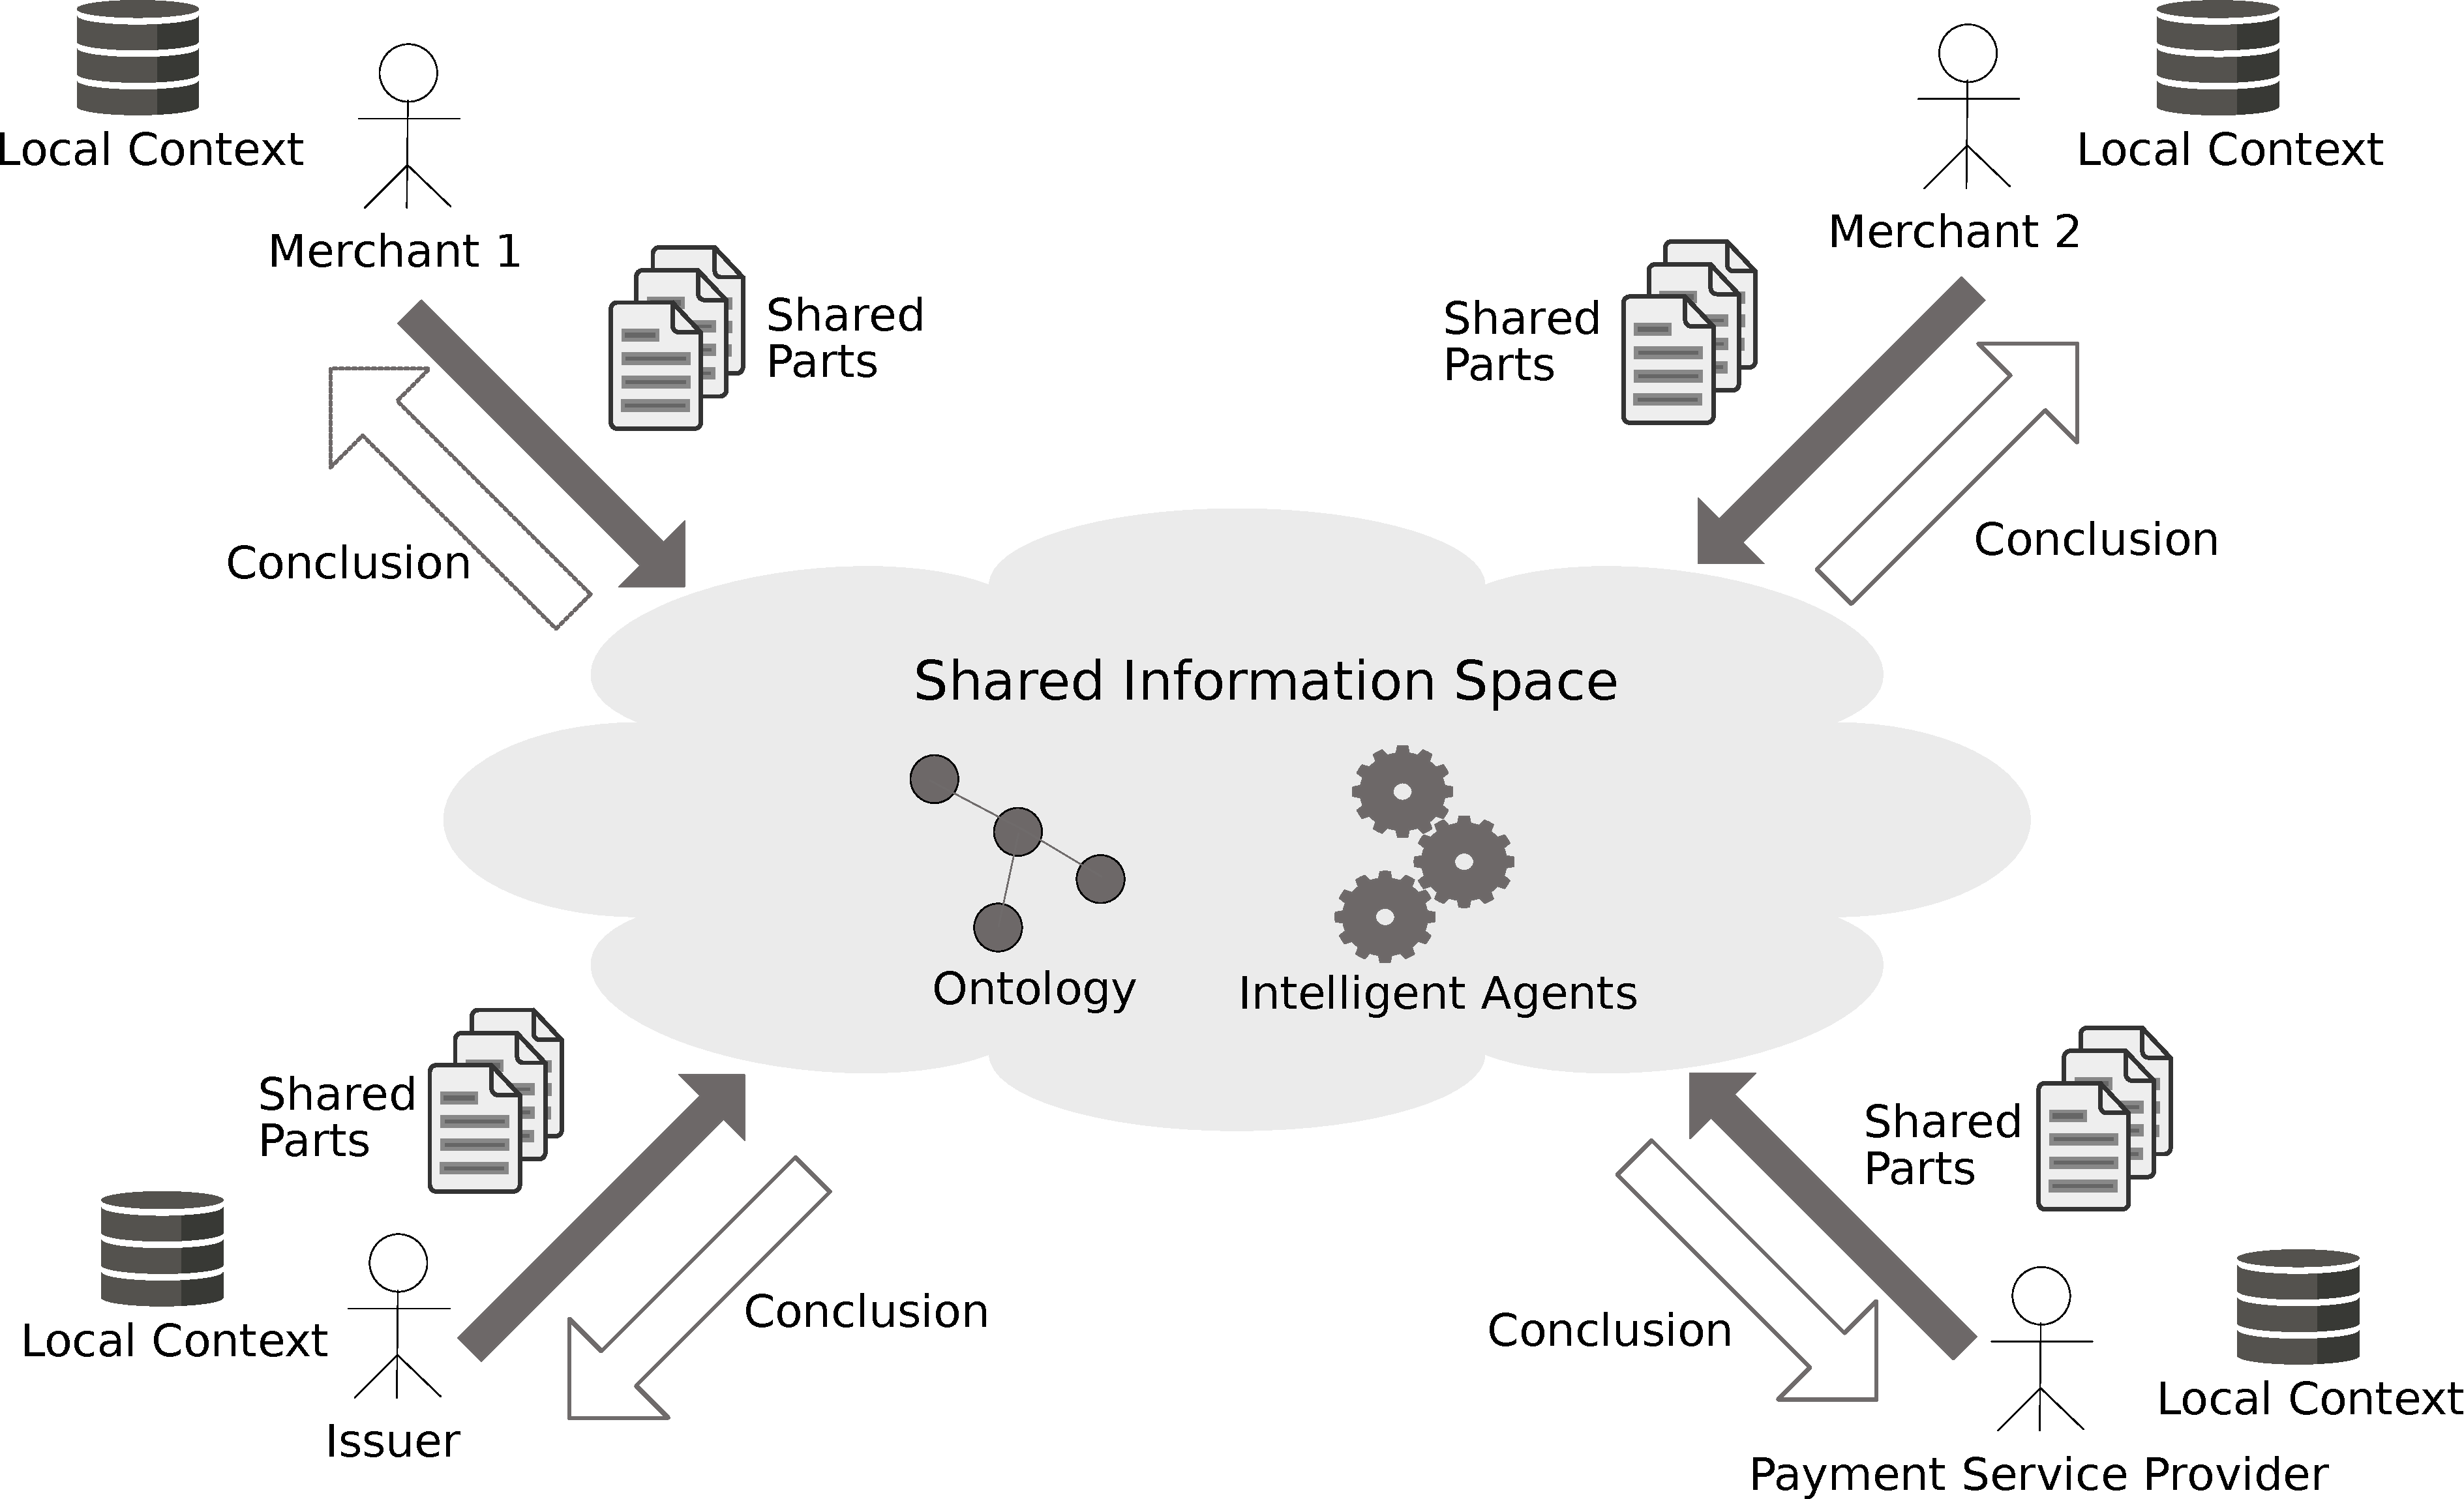
\includegraphics[width=0.9\columnwidth]{images/system_overview.pdf}
	\caption{High-level concept of the system}
\label{fig:images_system_overview}
\end{figure}

In this figure one can see, how the relevant parties provide access to parts of their internal local context information within a shared information space. The collaborative system should allow participants to communicate and collaborate on the \gls{E-commerce} fraud incidents from different places at the same time (see Section~\ref{sec:cscw}). Due to the fact that data from various sources have to be combined into a shared understanding of the \gls{E-commerce} activities of a consumer, there is a need to harmonise and transform the information from each participant into a common data model to be able to analyse the combined data set. Based on the shared understanding of the \gls{E-commerce} activities that have been done with a credit card recently, a set of intelligent agents (aka analysis tools) can assess them and present their findings, which can be valuable to any of the participants of the collaborative system.

% section concept_overview end


% sub chapter design data model
%!TEX root = ../MasterThesis.tex

\section{An \gls{ER} model for \gls{E-commerce} transactions}
\label{sec:data_model_transactions}

Based on the analysis of the information each stakeholder holds and transmits to others in Section~\ref{sec:stakeholder_analysis}, the following \gls{ER} model can be conducted for \gls{E-commerce} transactions (see Figure~\ref{fig:images_data_model}). This figure shows not only the relevant information from the local contexts of each stakeholder, but also how they can be combined within a shared information space. \\

\begin{figure}[!ht]
  \centering
  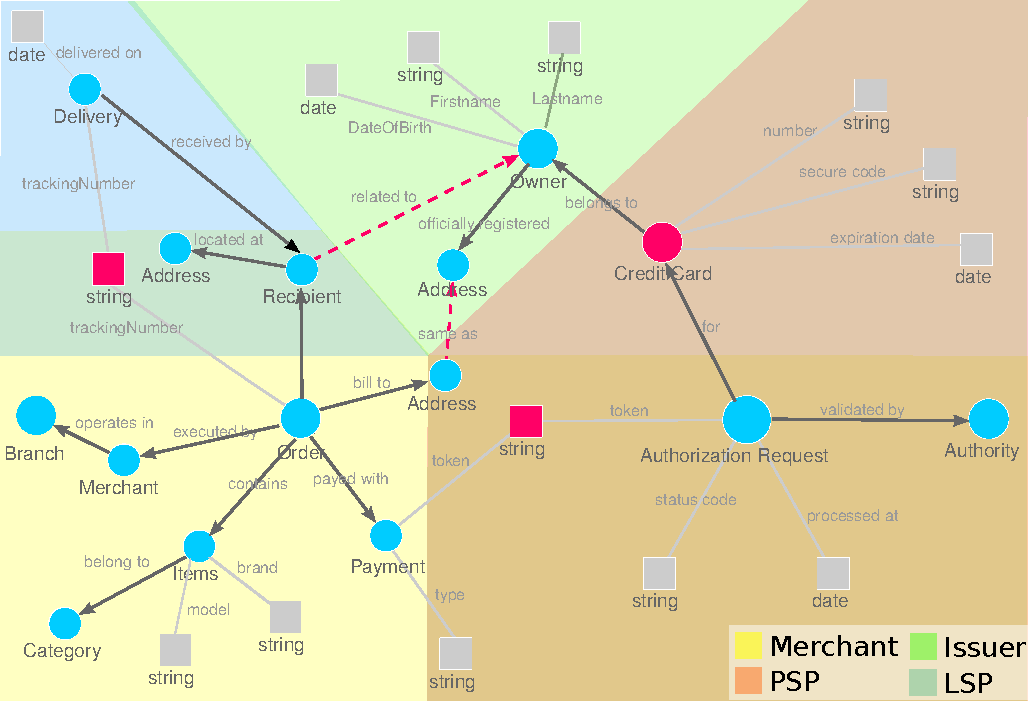
\includegraphics[width=0.9\columnwidth]{images/ontology_scenario_1.pdf}
  \caption[Entities and relations in the \gls{E-commerce} scenario]{Entities and relations in the \gls{E-commerce} scenario}
\label{fig:images_data_model}
\end{figure}

As the figure also shows there are \emph{shared information tokens} that will be exchanged between various stakeholders. Those can be used in the collaborative system as a reference for joining the distributed pieces of information into a combined view of an \gls{E-commerce} transaction. There are actually three important tokens: \@

\begin{enumerate}
  \item \textbf{payment token}: shared between merchants and \gls{PSP}s,
  \item \textbf{tracking number}: shared between merchants and \gls{LSP}s,
  \item \textbf{credit card}: shared between issuers and \gls{PSP}s
\end{enumerate}

In addition to these tokens Figure~\ref{fig:images_data_model} also shows the important validation criteria. These are two important connections that have an influence on the decision whether an \gls{E-commerce} transaction is evaluated as fraudulent or not. The two main criteria are: \@

\begin{enumerate}
  \item \textbf{billing address-to-owner address}: the billing address of the order has to match the registered address of the credit card owner
  \item \textbf{recipient-to-owner}: the recipient of the delivery has to be related to the owner of the credit card
\end{enumerate}

Whereas the first criteria can be examined during the payment authorization process of an \gls{E-commerce} transaction based on the information transmitted between merchants and \gls{PSP}s or issuers, the second one is more difficult to validate (or can not be verified at all). The only check the \gls{LSP}s are able to do, before they are handing over the packaged items to the recipients, is to verify that they are the ones mentioned in the shipping address information of the order. If a recipient is somehow related to the owner of the credit card used for paying an order, or just a deceiver misusing a credit card can not be confirmed by the \gls{LSP}. \\

Also merchants, \gls{PSP}s and issuers have no possibility to check for this criteria. Whereas the merchants are able to validate whether a consumer has send items to a shipping address before, they can not restrict consumers to choose only validated recipient addresses for their orders. Doing so would have negative impacts on the business success of the online merchant. The \gls{PSP}s and issuers can not analyse this situation either, because both participants will not receive any information about the delivery address of an order with the payment authorization request from a merchant. \\

But just sharing the fact whether the shipping and billing address of an order is different or not between the relevant stakeholders is not enough. Although this information is necessary, it is not sufficient to make a decision about suspicious transactions. Other necessary information are whether the consumer has send orders to this shipping address before, and information about the content of the current order. Nevertheless, as mentioned in Section~\ref{sec:scope_thesis} looking at the transactions of just one of the online merchants is not enough either to solve the \gls{E-commerce} fraud scenario, that this Master Thesis looks at. More sophisticated analysing capabilities are required for the collaborative system to be helpful for the \gls{E-commerce} fraud investigation.

% section system_overview (end)


% sub chapter design analysis
%!TEX root = ../MasterThesis.tex

\section{Analysis of \gls{E-commerce} transactions}
\label{sec:analyse_transactions}

Based on the explanations in the previous sections the proposal is to link the transaction information from various merchants, \gls{LSP}s, \gls{PSP}s and issuers together into a shared information space to be able to analyse, if there are any orders that look extraordinary, and are likely not being made by the owner of the credit card to a certain extend. Thus, the collaborative system has to use statistical evaluations and probabilities to find and rate suspicious activities. Starting with the credit card in question, an issuer can query for the order details of all the transactions that have been done recently with the credit card online. To be able to do that an issuer will likely have to query the \gls{PSP}s for the payment tokens first, before asking the affected merchants for order details to any of those payment tokens. At the end each online transaction can be mapped into an \gls{ER} model like the one shown in Figure~\ref{fig:images_data_model}, which resembles a large graph of entities and their relations, and has the specific credit card in the centre of it. An abbreviated sample graph of this procedure can be seen in Figure~\ref{fig:images_credit_card_graph}. \@

\begin{figure}[H]
  \centering
  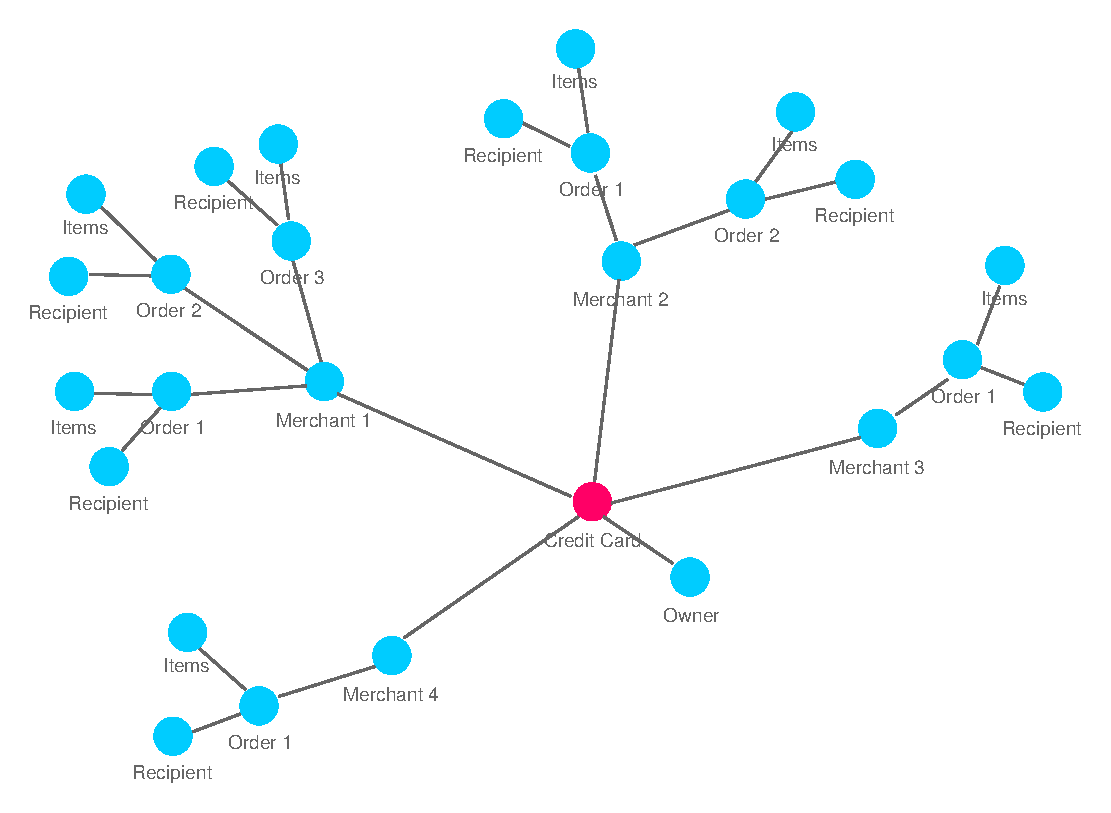
\includegraphics[width=0.8\columnwidth]{images/ontology_scenario_2.pdf}
  \caption{Building clusters of \gls{E-commerce} transactions by merchant}
\label{fig:images_credit_card_graph}
\end{figure}

As shown in this figure, the transactions will be organized by merchants first. But collecting the various order information into one combined data set is just the beginning of the \gls{E-commerce} fraud incident analysis. Based on the information received an issuer can already filter out transactions that have been shipped to different addresses than the one the credit card owner is registered for. Particularly for those edge cases it might be worth to ask for additional information from the affected merchants to be able to figure out, if the consumer has used one of these shipping addresses before. As a result the existing data set can be further enriched with supplementary transactional information from merchants at any time if needed. In addition to the address information an issuer can also analyse the item information (\gls{incl}\ category, brand and model) of each order to check for malicious activities. \\

But as already stated analysing the cluster of transactions on a merchant-by-merchant basis will not be sufficient to come up with a solid decision about a suspicious transaction. This is mostly due to the credit card usage pattern of the fraudsters, which has been explained in the scenario in Section~\ref{sec:scope_thesis}. Based on this description the various order details from the merchants have to be mapped and linked against each other, so that the initial graph of transactions, which is organized by merchant, can be easily transformed into complementary representations, which use different criteria to cluster the transactions such as recipient addresses, branches of merchants, or product-related information. \\

This reshaping of the transactional details can lead to new insights about the ``normal'' shopping behaviour of a credit card owner, and can make deviations from this behaviour visible. By using a clustered graph for visualizing the combined data set on screen, the exploratory nature of knowledge generation and perception will be supported, and so this kind of representation can help speed up the investigation of \gls{E-commerce} fraud incidents. An example visualization of a clustered graph, which groups information together based on a chosen criteria, is depicted in Figure~\ref{fig:images_graph_viz}. The different colours in this figure can represent different sources of information (e.g.\ \gls{E-commerce} transactions from various merchants). In this example information that stands out from the ``normal behaviour'' can be found in the top right and lower left areas of the figure. \@

\begin{figure}[H]
  \centering
  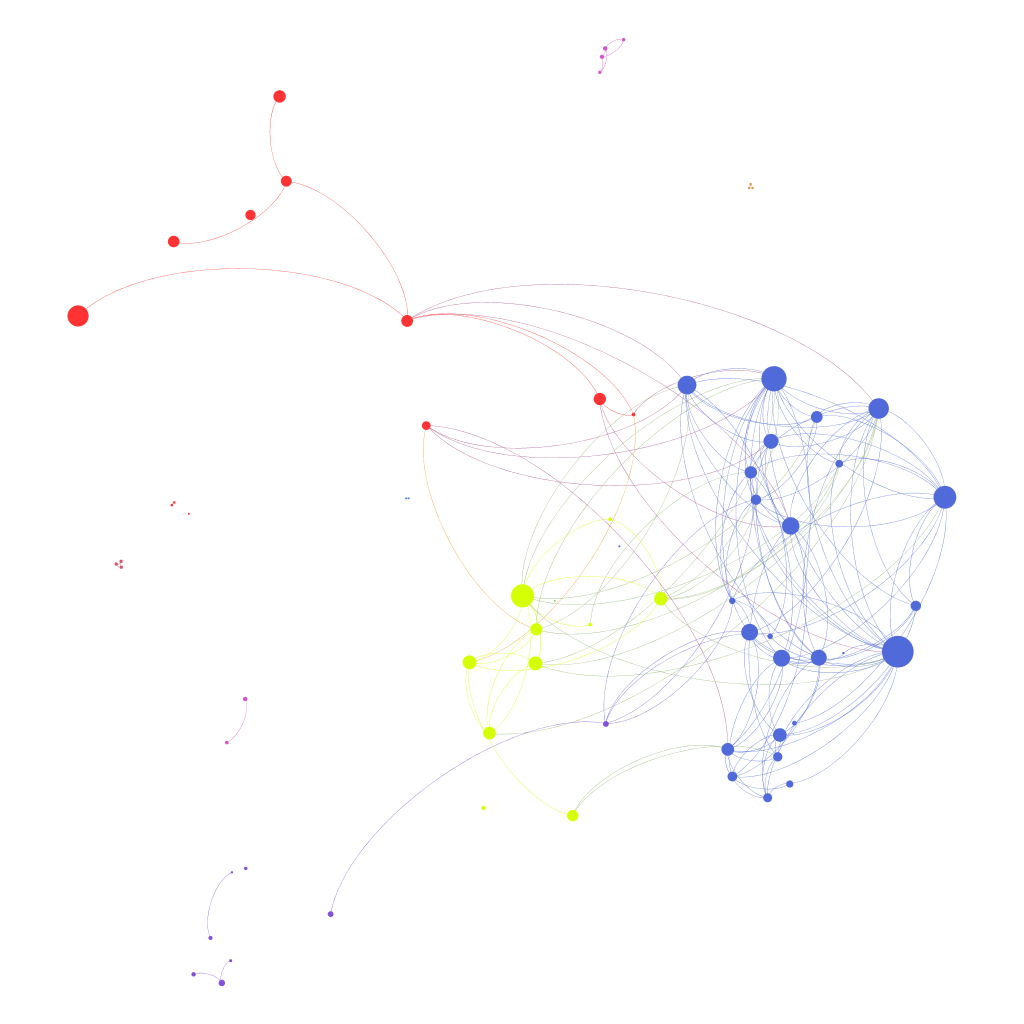
\includegraphics[width=0.8\columnwidth]{images/GraphViz.png}
  \caption[An example visualization of a clustered graph]{An example visualization of a clustered graph \citep{griffsgraphs}}
\label{fig:images_graph_viz}
\end{figure}

 In addition to these clustered graph visualizations the collaborative system can also support the \gls{E-commerce} fraud investigation by switching the type of representation based on the chosen criteria; e.g.\ when clustering transaction details based on location information such as shipping addresses, the system can present the information as a heat map on a chart as is displayed in Figure~\ref{fig:images_map_heatmap}. \@

\begin{figure}[H]
  \centering
  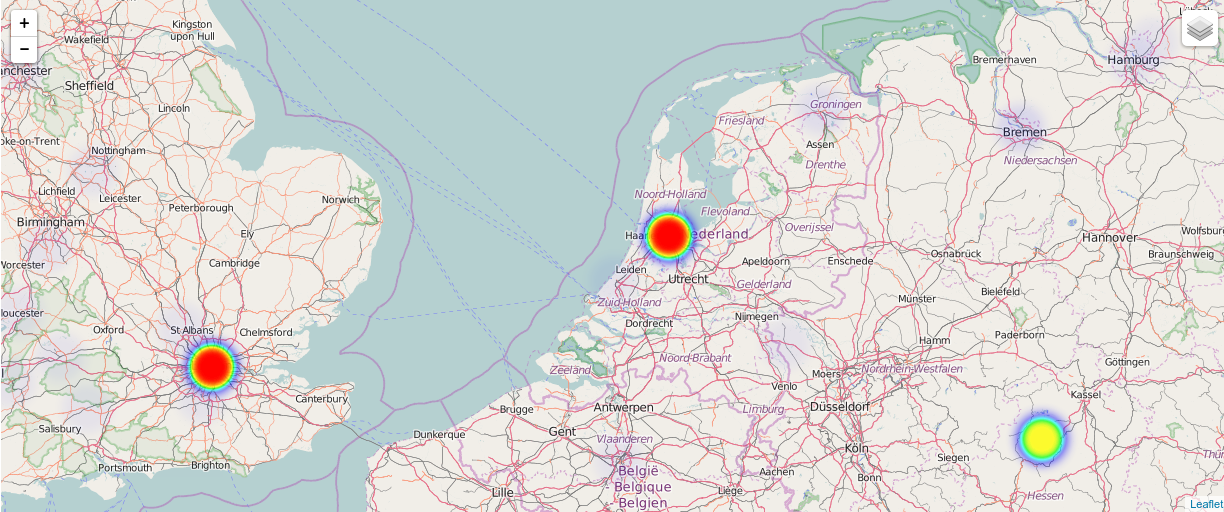
\includegraphics[width=0.9\columnwidth]{images/Heatmap.png}
  \caption{Heatmap displaying clusters of location-based information}
\label{fig:images_map_heatmap}
\end{figure}

Additionally, the collaborative system can provide a Hypertext-based visualization of the \gls{E-commerce} transactions to allow investigators navigating through the consolidated order details done with a credit card recently. \\

To sum up the system have to support the collection and combination of \gls{E-commerce} transaction information from various sources into a linked data set using a graph-oriented data model. This graph can further be analysed from multiple view points to validate, if there are any transactions that stand out from the ``normal'' shopping behaviour of the credit card owner. The starting point for the investigation is a sequence of payment tokens of recent credit card activities that an issuer can provide to the \gls{PSP}s. The linked data set will initially collect and cluster the information from each merchant based on this list (see Figure~\ref{fig:system_workflow}). In case there are already suspicious information in one of these clusters, an issuer can ask for further details and enrich that specific cluster with additional order information for this consumer and that merchant. In the final step the system has to do the mapping and linking of the order detail information between each merchant to allow subsequent analysing and clustering of the transaction details based on various criteria.

\begin{figure}[H]
  \centering
  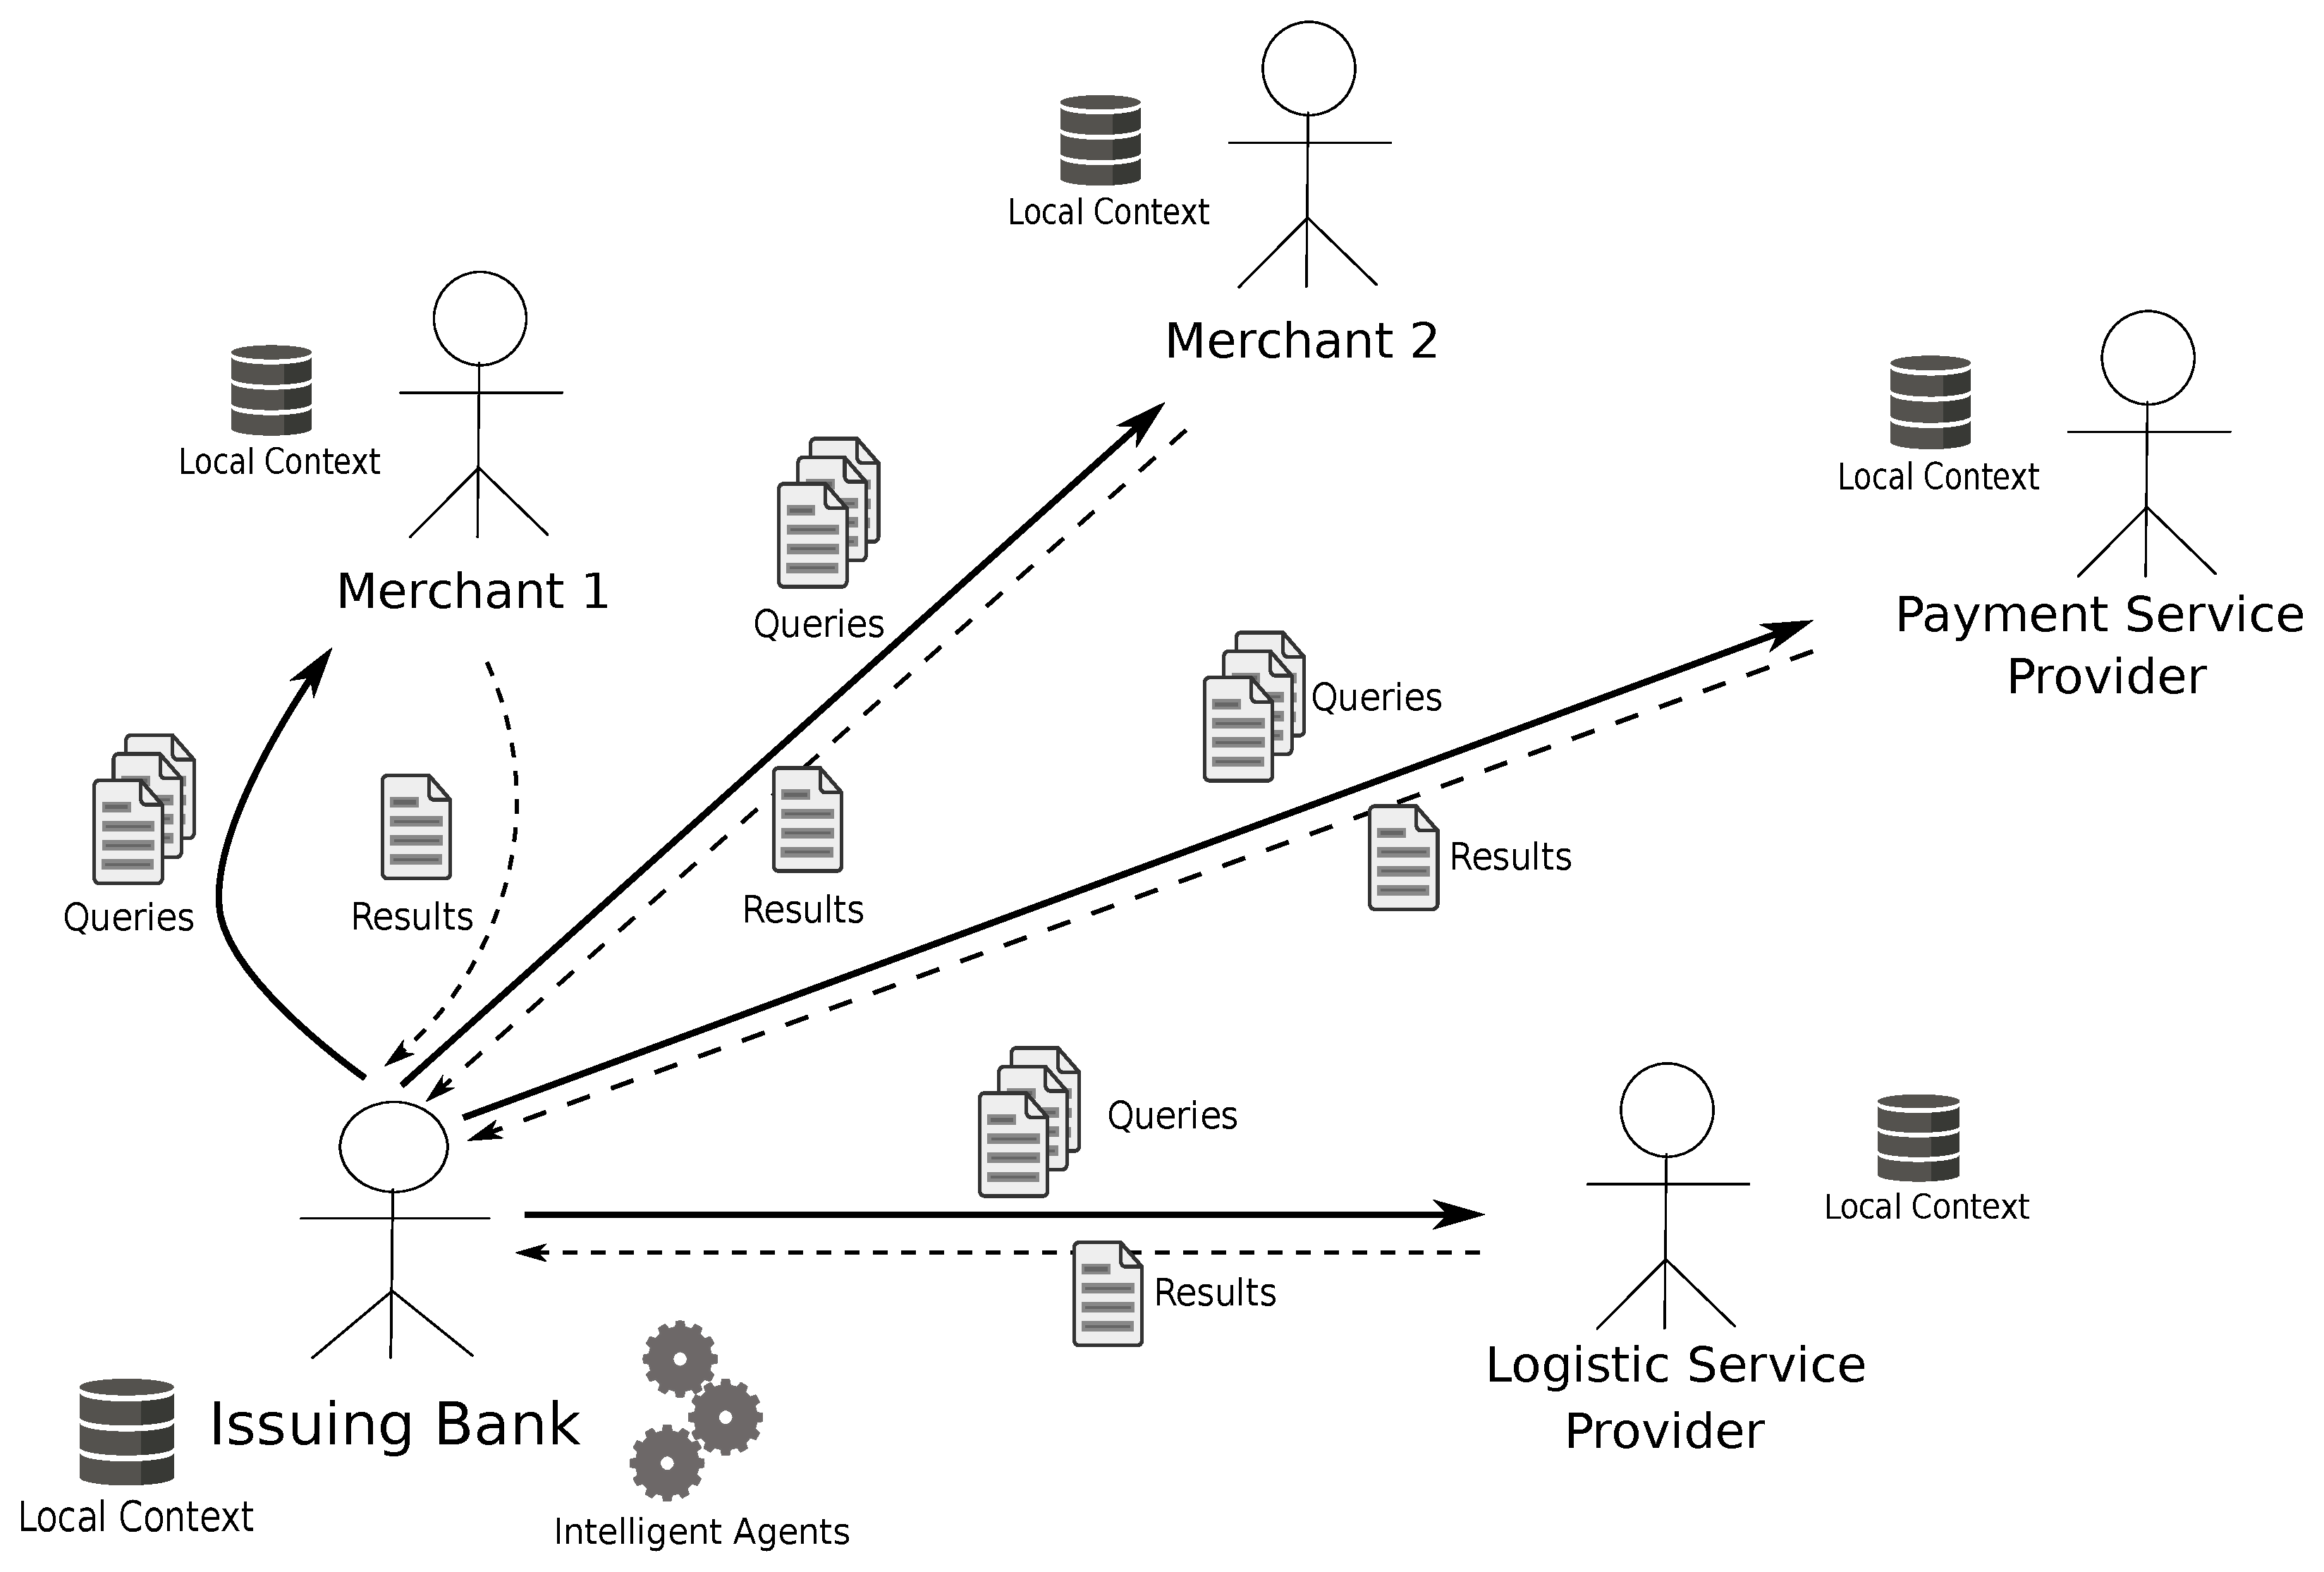
\includegraphics[width=0.7\columnwidth]{images/system_P2P_decentralized.pdf}
  \caption{Information flow in the proposed collaborative system}
\label{fig:system_workflow}
\end{figure}

% section system_overview (end)


% sub chapter existing approaches
%!TEX root = ../MasterThesis.tex

\section{Evaluation of existing design approaches}
\label{sec:system_approaches}

When trying to solve issues of information integration between organizations there are already existing solutions, which have to be examined whether they might fit the \gls{E-commerce} fraud investigation scenario or not. This section looks into common existing approaches to collect and integrate information between \gls{IT} systems.

\subsection{\gls{ETL} processes}
\label{subsec:etl_process}

To begin with, retrieving, transforming and combining data from multiple dispersed data sources is not a completely new problem, and is actually part of ``Extract-Transform-Load'' (\gls{ETL}) processes \emph{within} an organization. The basic idea is very much the same as in the concept shown in this thesis; namely to get as much information as possible from the various databases that are in use within a company, harmonise (aka transform) the data from each of them into a shared data model, and use the cleaned up and combined information repository for doing advanced business analysis and predictions later. Data within an organization is created and maintained by different business-related software tools. Each of these will usually store the information into their own database using a vendor-specific database schema. Other business-relevant information might be stored in structured files, sometimes using a proprietary format such as Microsoft Excel. Each of these data sources have to be accessed, the valuable information have to be extracted and mapped against each other, before the analysis of it can begin in a separate data store that holds the combined data set. The whole process is visualized in Figure~\ref{fig:images_etl_process}. \@

\begin{figure}[H]
  \centering
  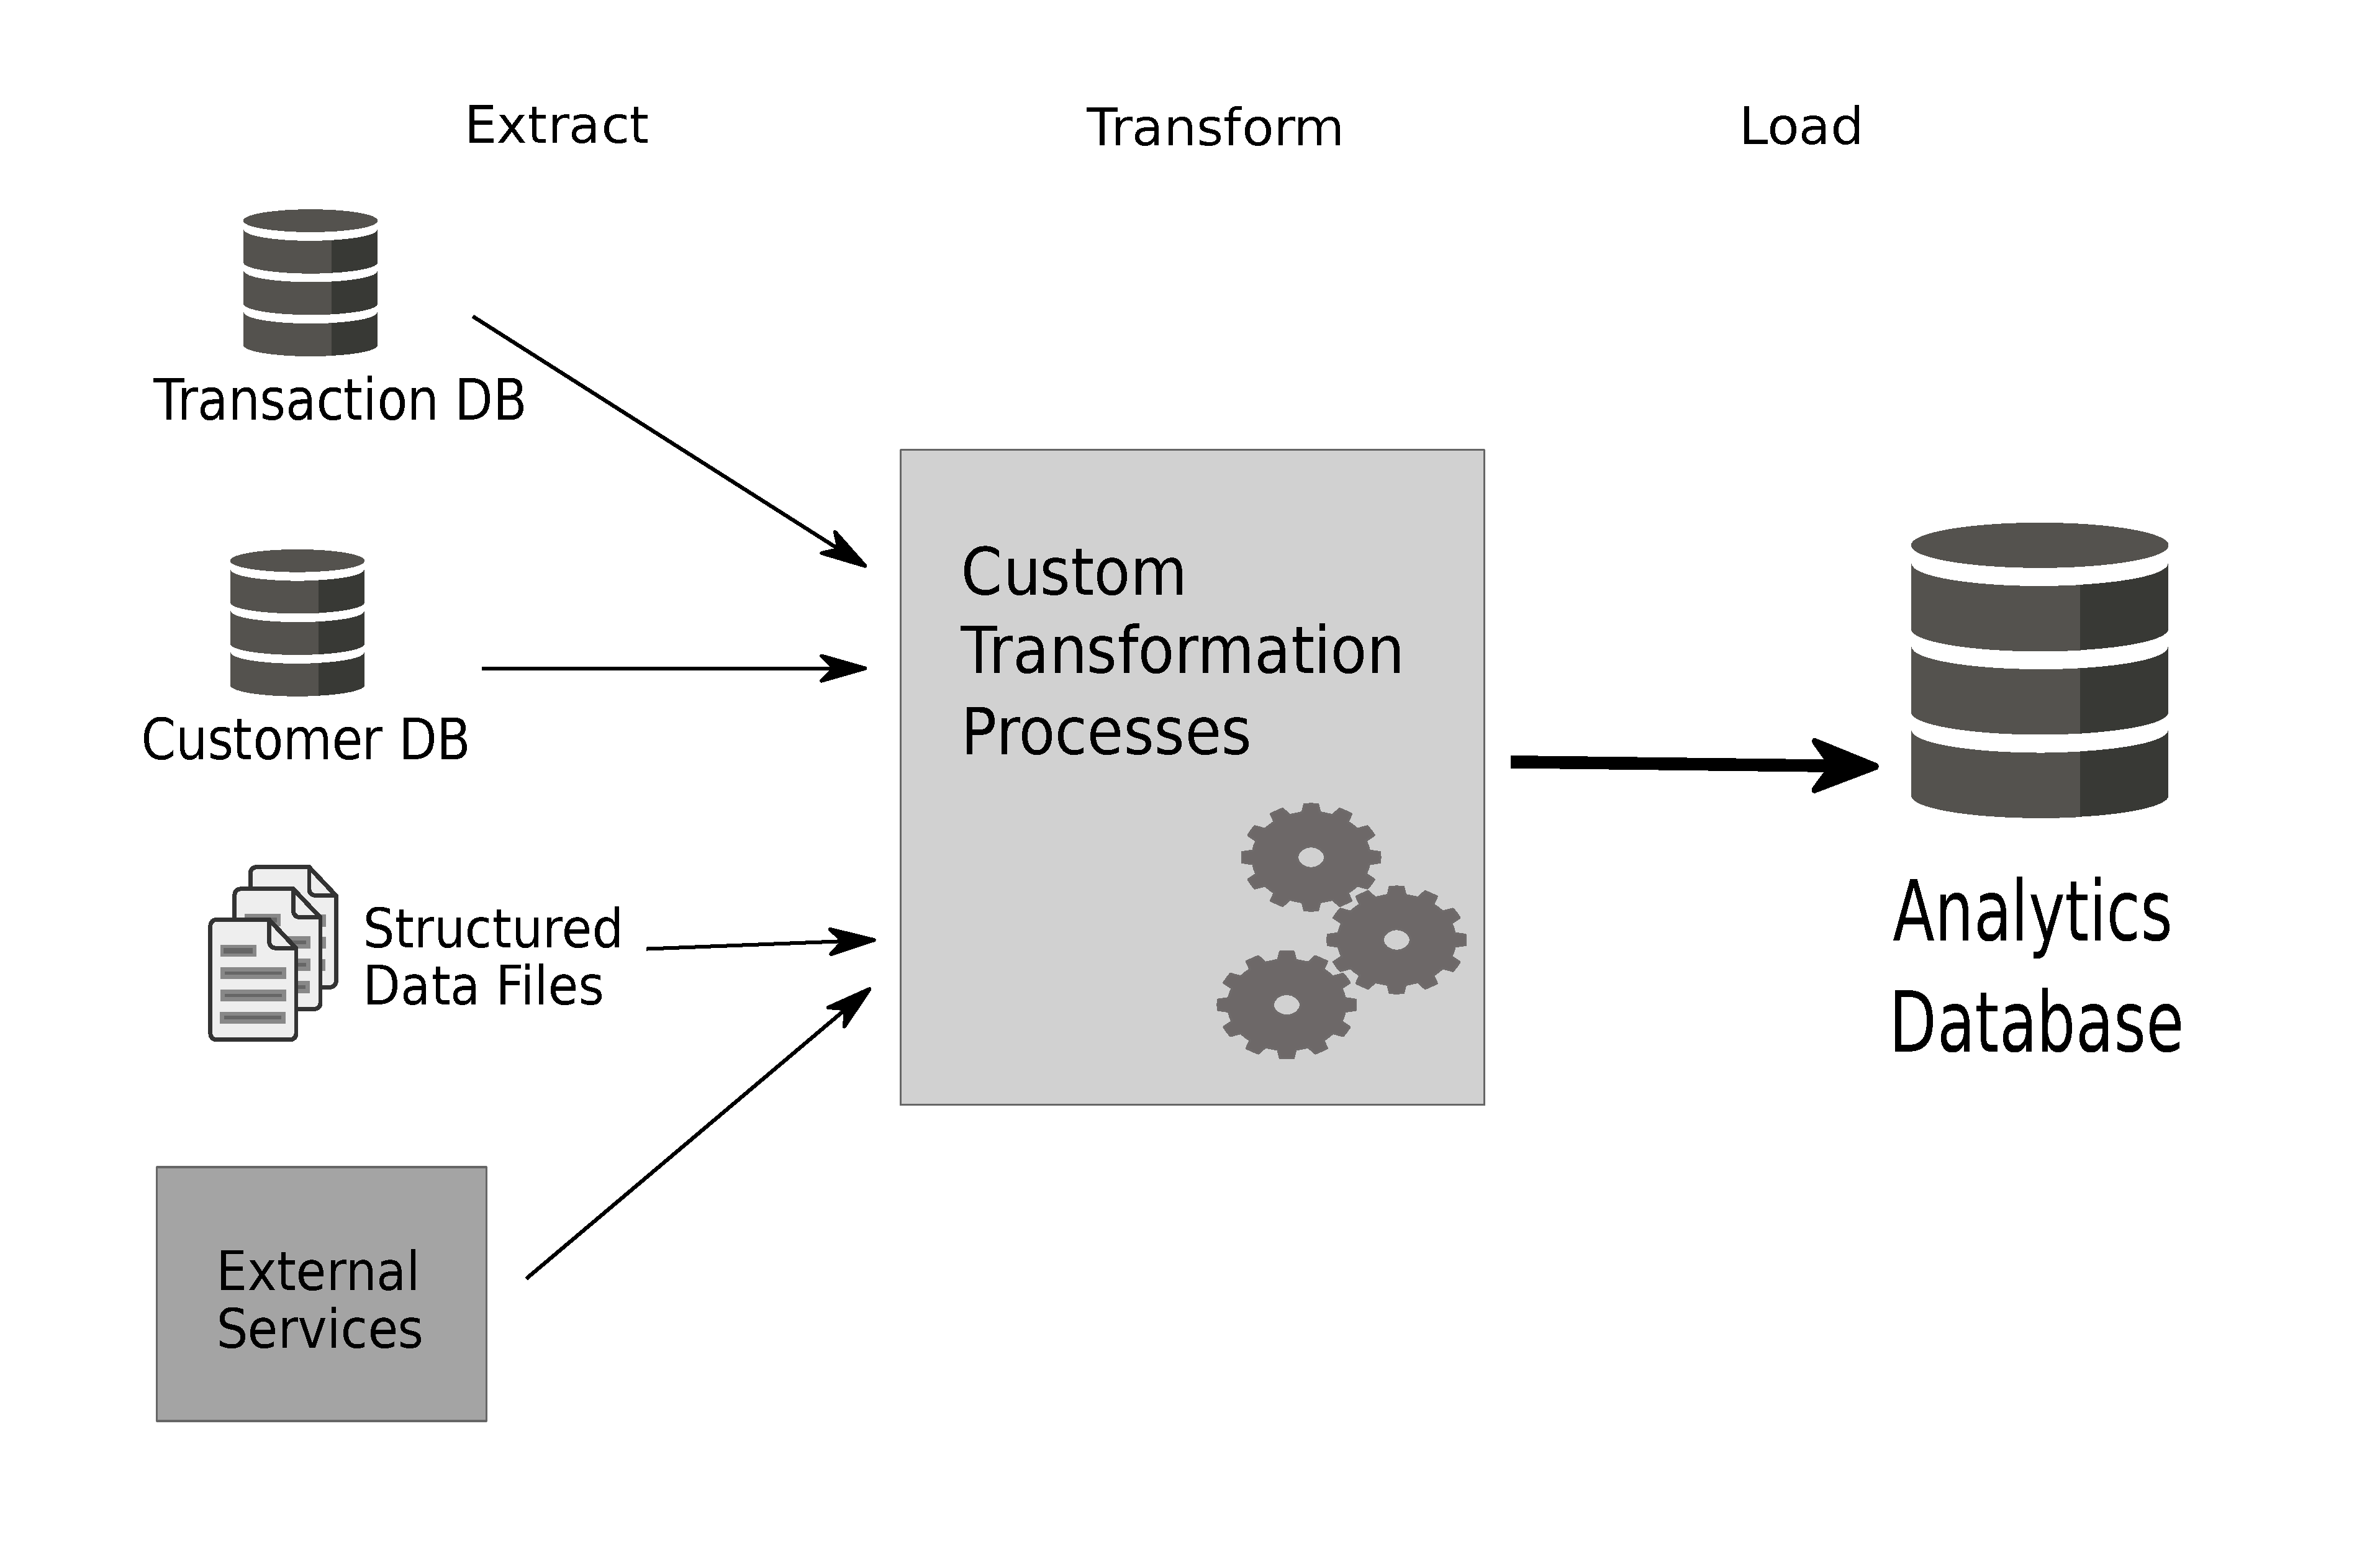
\includegraphics[width=0.9\columnwidth]{images/etl_process.pdf}
  \caption[ETL process within a company]{\gls{ETL} process within a company \citep[pg. 165]{wood2014linked}}
\label{fig:images_etl_process}
\end{figure}

Although this description basically resembles the required activities as explained in the conceptual overview of the \gls{E-commerce} fraud investigation system before, these \gls{ETL} processes generally rely on an in-depth knowledge of the data structures that are used in each of the information sources, as well as require a direct access to the databases and files for retrieving the information. Although these preconditions are not cumbersome to work with \emph{within} an organization, they are not suitable for situations, in which one has to integrate data sources across company boundaries. As the integration of the information takes place on the database level, granting external partners access your internal databases will not only open up access to your business internals, but will also make it much more complicated to change the underlying database structures and business-related software tools later. Any changes to one of these would require elaborate negotiations between the owner of a data source and all of the external partners depending on it. \\

Beside these drawbacks, which make the \gls{ETL} approach unsuitable for the \gls{E-commerce} fraud investigation scenario as a whole, one can assume that these \gls{ETL} processes are still in use for operating the daily business of each stakeholder involved. They can be helpful in the discussion later (see Section~\ref{sec:working_semantic_data}) when a decision has to be made about how each stakeholder can prepare and transform his internal data sources for external consumptions.

% section etl_process

\subsection{Web Services}
\label{subsec:web_services}

With the development of the \gls{E-commerce} scenario there was also a need to integrate business functionalities from various service providers on the Internet. Valid examples for these kind of integrations are the usage of the \gls{PSP}s for doing the payment as well as the \gls{LSP}s for handling the shipping process. These approaches resulted in the ``Service Oriented Architecture'' paradigms, which enable application services provided by different vendors to talk to each other via a public facing programming interface (aka \gls{API}). The only requirement for such interoperability to work properly is that each public interface follows some standardized or commonly agreed upon guidelines to be vendor-, platform- as well as programming language-agnostic. One possible implementation of these concepts are the so-called \emph{Web Services}, which use the WS* protocols and standards from the \gls{W3C} with the extensible markup language (aka \gls{XML}) and the \gls{HTTP} protocol at their core \citep{josuttis2007soa}. \\

Like the \gls{HTML} format, which is used to represent Web pages on the Internet, \gls{XML} is originally based on \gls{SGML}, but instead of formalizing markup tags for structuring and styling textual content it is a meta-language allowing everyone to define their own markup languages. In this matter it doesn’t dictate what tags are available to structure the information; instead it includes some basic guidelines for creating well-formed and valid documents that uses domain-specific tags, which can be freely defined and structured by the creator of the \gls{XML} document. Therefore it is better suited in situations, in which a computer has to parse and evaluate the content of a message; assuming the computer program knows the structure of that message. In an additional step the author of the \gls{API} could also specify an \gls{XML} schema for each message, which describes the structure of the message with all the possible elements, their ordering, nesting level and data types in detail. By doing so the \gls{XML} parser program can later verify the content of a message received against the \gls{XML} schema, and validate if it is a valid document related to that schema definition. \gls{XML} schemata are also expressed in \gls{XML} format and have been standardized by the \gls{W3C}. \\

Being able to create custom markup languages via \gls{XML} has a huge benefit for machine-to-machine communication and is the basis for integrating Web Services (via the WS* protocols), but it still has limitations when it comes to figure out the semantics of those \gls{XML} messages. This is mostly due to the fact that each \gls{XML} document represents a new markup language and needs a specific \gls{XML} parser to be understood by the machine; also to distinguish commonly used tag names in an \gls{XML} document the creator has to place them into specific namespaces (aka \gls{XML} namespaces). But these \gls{XML} namespaces further complicate the automatic processing of \gls{XML} documents and increase the necessity to have custom instances of \gls{XML} parsers for each \gls{XML} document \citep{taylor2008p2p}. \\

An integration of information exchanged via Web Services is therefore handled separately for each Web Service interface. Looking at the payment service integration as \emph{one} possible example, the following steps are necessary to allow a merchant to interact with the Web Service of a \gls{PSP}: \@

\begin{itemize}
  \item the \gls{PSP} has to define and implement an interface (aka \gls{API}) that a merchant can use for exchanging information,
  \item the \gls{API} includes a set of request/response messages that hold the data being exchanged, usually specified in \gls{XML} format, as well as a list of operations that the interface supports,
  \item the \gls{PSP} has to document each of these messages and operations, \gls{incl}\ their intended structures and semantics,
  \item the \gls{PSP} has to provide access to the \gls{API} via an \gls{HTTP} endpoint running on a server at a specific \gls{URL},
  \item the \gls{PSP} usually restricts access to this interface for registered partners only; for doing so they have to provide a registration and identification mechanism,
  \item the merchant has to register with the \gls{PSP} to be able to call into the Web Service \gls{API},
  \item the merchant receives some kind of token that can be used to identify with the Web Service later,
  \item the merchant has to implement an \gls{API}-specific client-side wrapper that knows how to talk to the interface; \gls{incl}\ calling one of the available operations as well as serializing and de-serializing the messages, which will be transmitted between the Web Service and the client program,
  \item the client program from the merchant has to understand the structures and semantics of the messages exchanged with the Web Service and react on them accordingly.
\end{itemize}

Although other merchants, who want to use the same \gls{API} from the \gls{PSP}, can use the same client-side wrapper, which is sometimes also provided by that \gls{PSP} for convenience, to be able to send/receive messages to/from this specific Web Service, they still have to make the \gls{API}-specific integrations into their own Web shops. Also these integrations are only done in an \emph{one-way} direction. To allow the merchants to provide information from their own databases, the merchants have to do likewise and provide an \gls{API} that others can use to query for information by following the same steps as mentioned above. \\

Additionally, as the structures and semantics of the messages and operations of each Web Service interface are not standardized, integrating with \gls{API}s from other \gls{PSP}s or issuers result in doing the same integration steps again and again. To make things worse, the mapping and linking of the information coming from different \gls{API}s have to be implemented by each client to be able to analyse the combined data sets. It becomes clear soon that these necessary tasks will increase the time and efforts with each additional stakeholder, who wants to participate in the collaborative system, see Figure~\ref{fig:web_services_scenario}. \\

\begin{figure}[!ht]
  \centering
  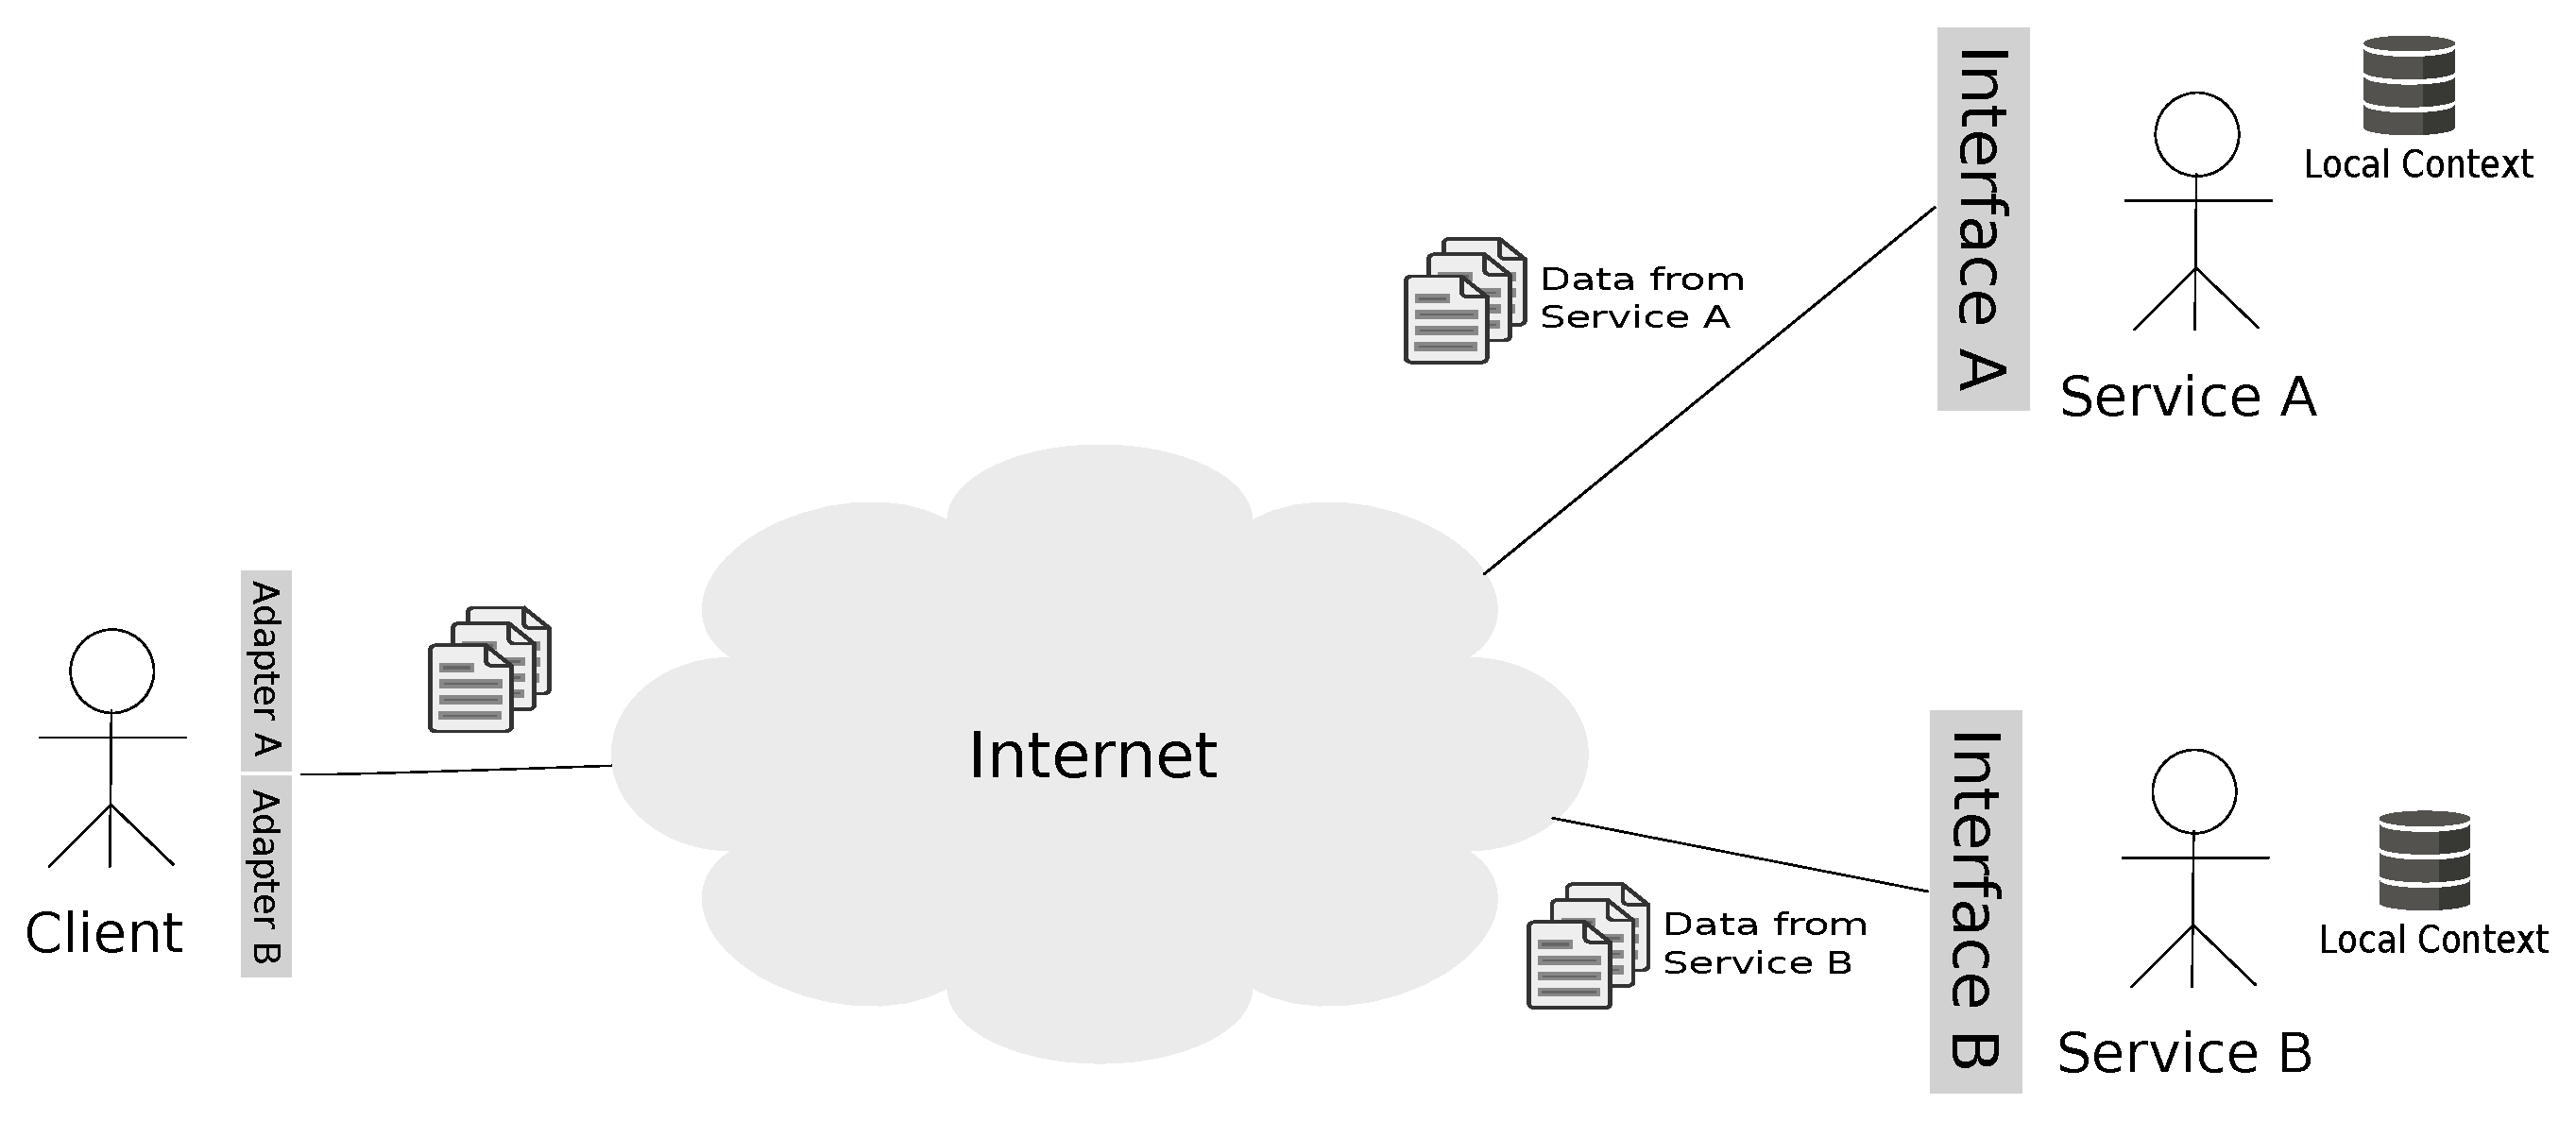
\includegraphics[width=0.9\columnwidth]{images/web-services-scenario.pdf}
  \caption{Data integration within the Web Service approach}
\label{fig:web_services_scenario}
\end{figure}

As conclusion one could say that integrating information between a larger group of participants is very limited with the existing Web Service approach. The steps necessary for exchanging information result in huge efforts on all participating parties. As there is no common way to access and combine the information from each of the participants, beside using the fundamental \gls{HTTP} protocol and \gls{XML} data format, there have to be a lot of collaborative work between each of them upfront to come up with an approach for integrating the available \gls{API}s, and provide the rules for combining the different data structures. Due to these restrictions one can assume that an integration based on the Web Service approach will only work well with a limited number of participants. This might lead to a collaborative system that will only include larger online merchants, \gls{PSP}s and issuers as participants, and therefore left out smaller companies from the \gls{E-commerce} fraud investigation process. For a general solution of the problem described in Section~\ref{sec:scope_thesis} this is not sufficient. Due to these limitations one will need other technologies that provide a better scalability and integration ability for the exchange of information between various, otherwise not strongly related organizations.

% subsection web_services (end)

\subsection{Semantic Web}
\label{subsec:web_data}

``The Web is full of intelligent applications, with new innovations coming every day'' \citep{allemang2011semantic}. But each of these intelligent Web applications are \emph{solely} driven by the data available to them. Information that are likely coming from different places in the global information space, accessible usually \emph{only} via a custom \gls{API} on the server hosting those resources (see Section~\ref{subsec:web_services}). But the more consistent the information available to the smart Web application are, the better the service and its result will be. To support an integration of the data from various Web services, the semantics of the information delivered by each of them have to be available, and there has to be a generalized, formalized way to express the semantic of that data. The focus on a standard, which enables Web services to express the semantics of the data, also allows for global scalability, openness and decentralization that are the key principles of the World-Wide Web. The \emph{Semantic Web} tries to give a solution for this problem by providing the Resource Description Framework (aka \gls{RDF}) and related technologies (e.g. \gls{RDF} schema, \gls{SPARQL}, \ldots) for describing, linking and querying the data that a Web service delivers. But it doesn’t reinvent the wheel; instead the Semantic Web builds upon existing, proven technologies such as \gls{XML}, \gls{XML} namespaces, \gls{XML} schemata, and the \gls{URI} to uniquely address resources on the Web \citep{allemang2011semantic}. \\

The main benefits of the Semantic Web approach are the specification of a standardized and generalized format to exchange information on the Web (aka \gls{RDF}) as well as a commonly agreed way to access and query for them (aka \gls{SPARQL}). The \gls{RDF} data format does not only specify the syntax of the information exchanged, but also include the semantics (aka meanings) of them. Due to this fact resources described in \gls{RDF} format are consistent and semantically self-contained. These characteristics are achieved by providing information as a triple; that is a statement consisting of the resource in question (aka subject), a predicate and the specific value (aka object) for it. To be able to unambiguously identify the meaning of these statements, each part of such a triple is usually expressed with a unique \gls{URI}. These \gls{URI}s can be abbreviated via ``prefix'' definitions to make the whole statement easier to read (see also Section~\ref{sec:semantic_web}). To specify that there is an order ``12345'' from a ``merchant1'', one can come up with the following \gls{RDF} statement, which uses the Schema.org \gls{RDF} vocabulary \citep{Schema.org} to describe an order: \@

\begin{listing}[H]
  \inputminted[linenos,
               numbersep=5pt,
               breaklines=true,
               frame=lines]{TURTLE}
               {./samples/sample_order_12345.ttl}
  \caption{An order specification in \gls{RDF}}
\label{lst:sample_order_ttl}
\end{listing}

An \gls{RDF} file can contain one or more of such triples describing the resources of interest in detail. Usually these triples are visualized as directed graph, in that subjects and objects are displayed as nodes and their predicates as edges between them. The order resource shown in the Listing~\ref{lst:sample_order_ttl} above can also be visualized as directed graph as shown in Figure~\ref{fig:sample_order_graph_image}. \@

\begin{figure}[H]
  \centering
  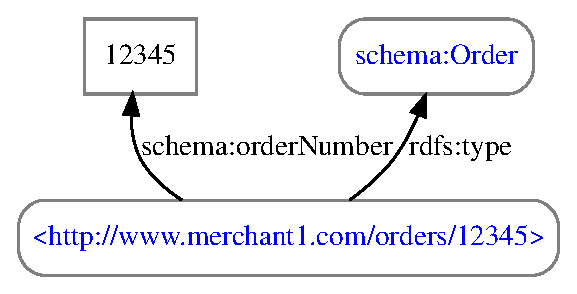
\includegraphics[width=0.6\columnwidth]{images/sample_order_12345.pdf}
  \caption{Graph-based visualization of the order from Listing~\ref{lst:sample_order_ttl}}
\label{fig:sample_order_graph_image}
\end{figure}

Additionally, the \gls{RDF} format has build-in support for merging information from different data sources. This functionality is only working as expected if the triples in the dispersed data stores are using the same \gls{URI}s to refer to the same subjects or objects. In that situation merging the triples from different \gls{RDF} data sets will result in a locally linked data set holding the combined information as shown in Figure~\ref{fig:images_combine_rdf_graph}. \@

\begin{figure}[H]
	\centering
		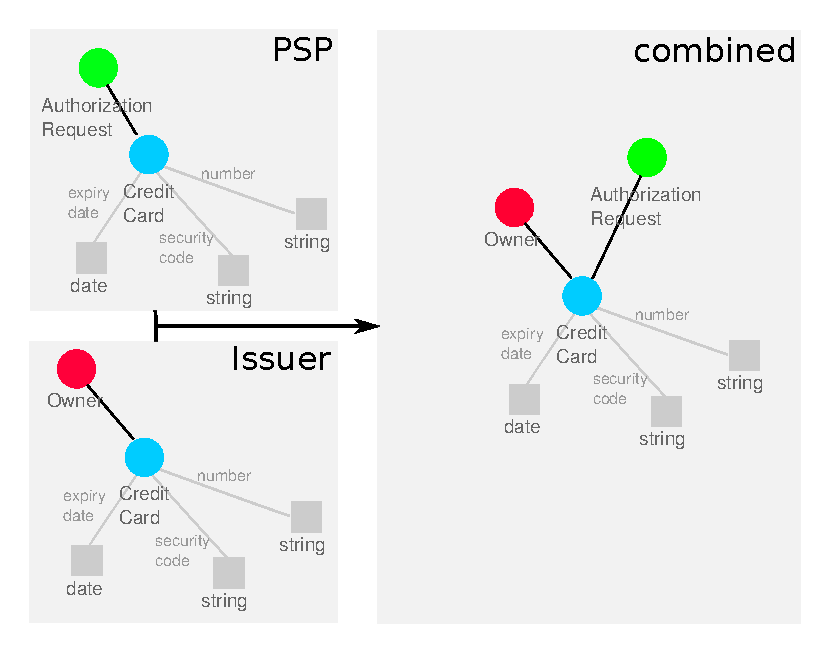
\includegraphics[width=0.9\columnwidth]{images/combine_rdf_graph.pdf}
	\caption{Combining two \gls{RDF} files containing the same credit card entity}
\label{fig:images_combine_rdf_graph}
\end{figure}

Beside being able to provide internal resources in an understandable \gls{RDF} format for external consumption, the Semantic Web also specifies how to query and access these ``information databases'' on the Web. For that purpose the \gls{SPARQL} protocol and query language has been defined. It does not only describes a language to query for information located in \gls{RDF} data stores, but also specifies how to setup an \gls{HTTP} endpoint on a server to make the \gls{RDF} data set publicly available on the Internet. \\

Following the specifications of the Semantic Web standards each relevant participant of an \gls{E-commerce} fraud investigation system will have to transform the information from their internal databases into a set of triples with commonly agreed upon \gls{URI} references and persist them into a \gls{RDF} data store. For this transformation process an extension of the existing \gls{ETL} processes in an organization can be used. Additionally, these \gls{RDF} data sets will be made available publicly on the Web for information retrieval via the \gls{SPARQL} protocol and query language. Each participant of the collaborative system will only need to know the specific addresses of these \gls{HTTP} endpoints to be able to query them for information. The results of each query can be easily combined into a local \gls{RDF} data set based on the merging capabilities of the \gls{RDF} standard. This will decrease the efforts for integrating the data from various external sources drastically. Also communicating with the different \gls{HTTP} endpoints to access and query for information is being done in a much more efficient way based on the standardized \gls{SPARQL} protocol and query language, see Figure~\ref{fig:web_data_scenario}. \@

\begin{figure}[H]
  \centering
  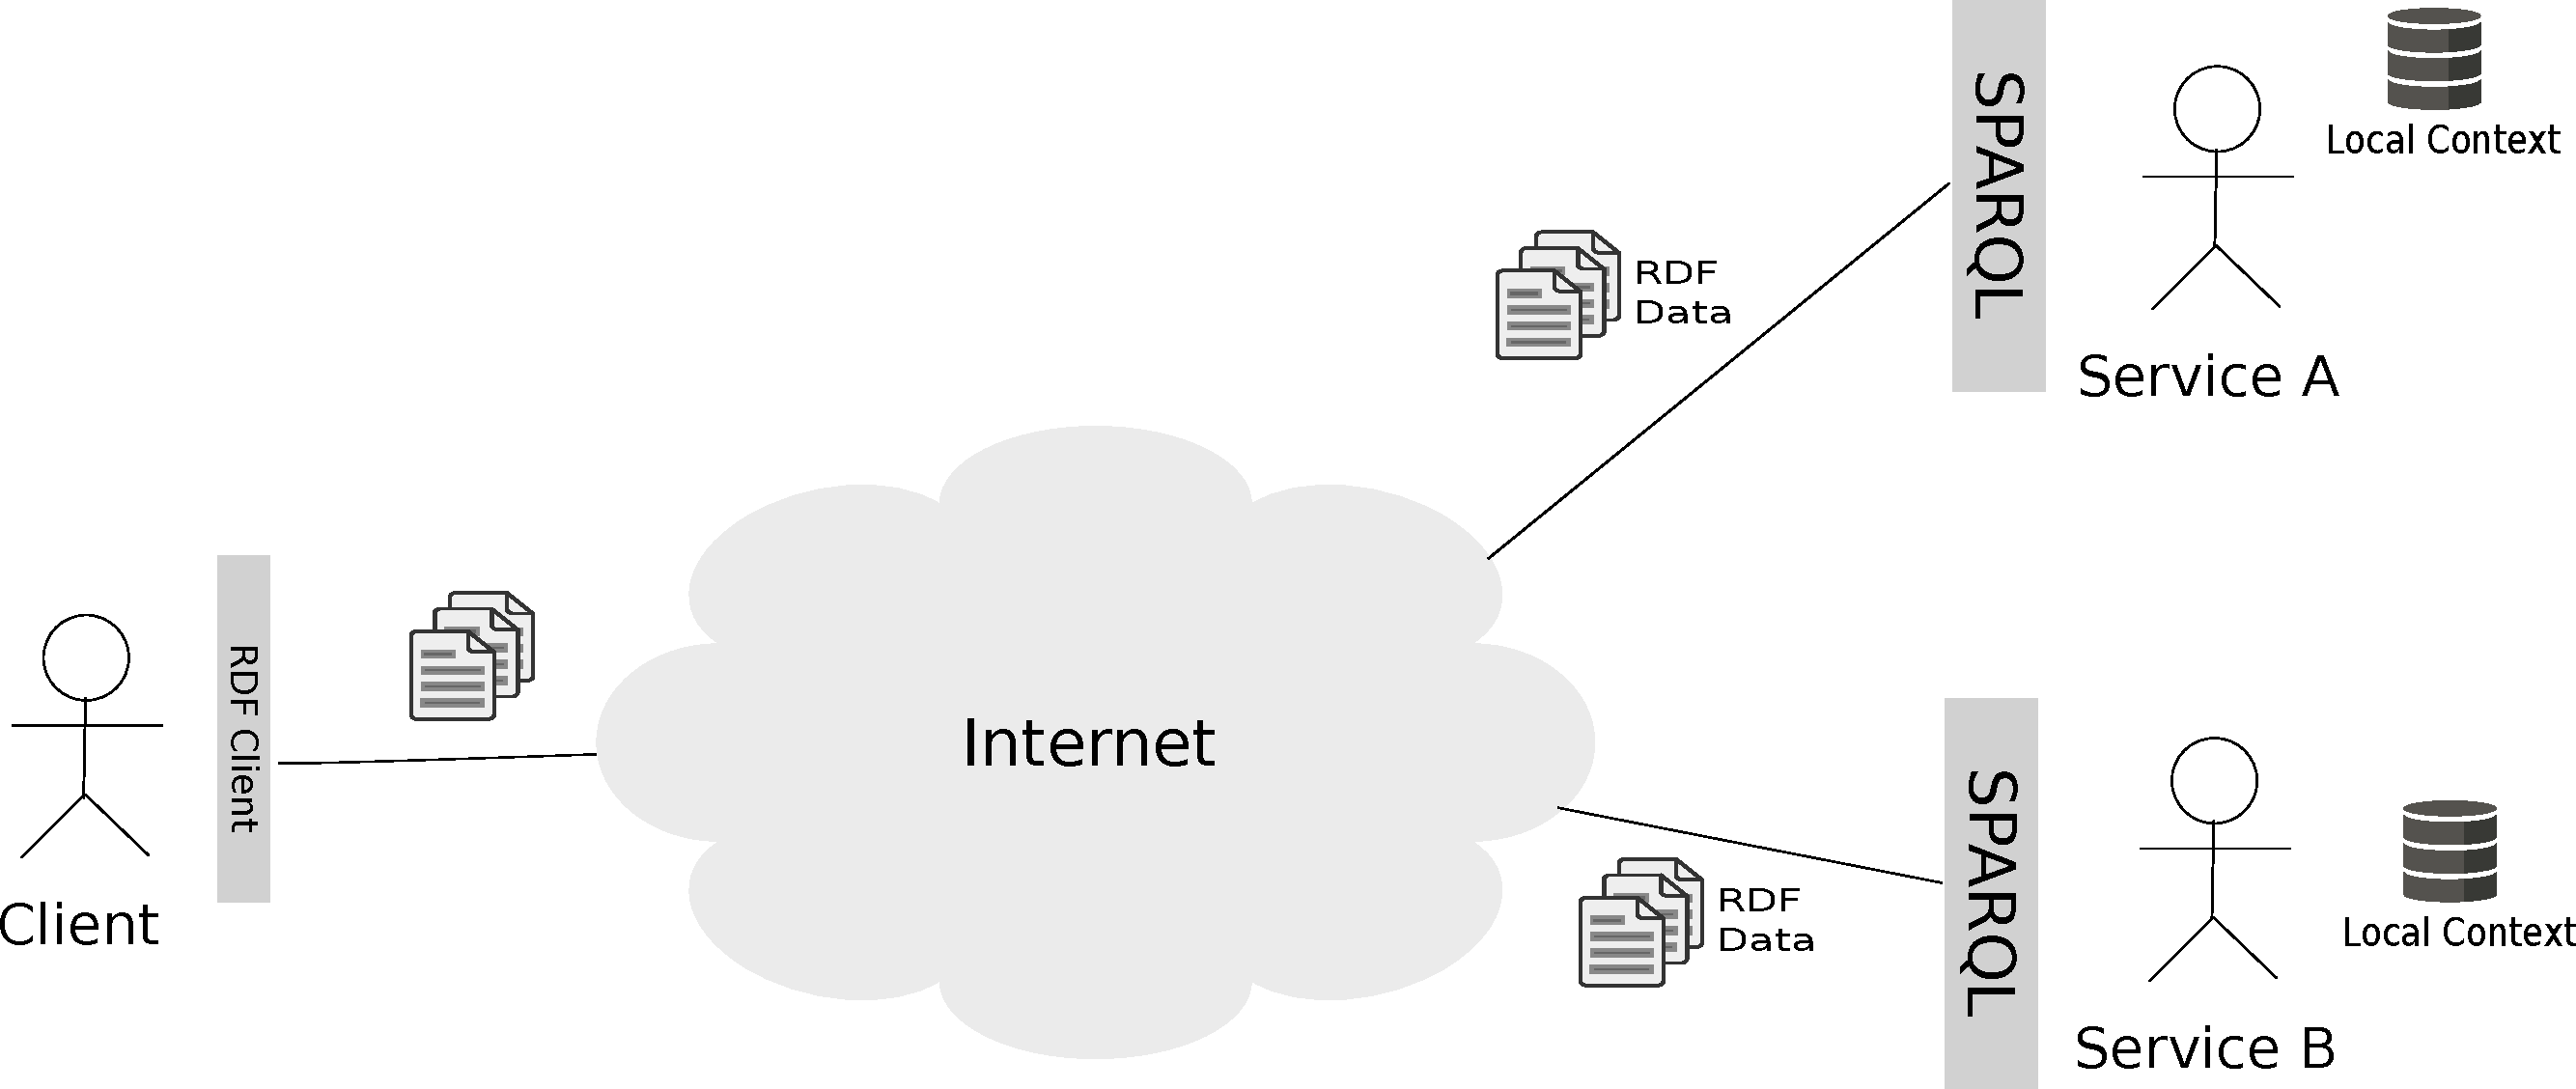
\includegraphics[width=0.9\columnwidth]{images/web-data-scenario.pdf}
  \caption{Data integration within the Semantic Web approach}
\label{fig:web_data_scenario}
\end{figure}

As the underlying model of a \gls{RDF} data set is resembling a graph-based data model it will fit the concept of the proposed system from Section~\ref{sec:analyse_transactions} perfectly. Still requiring every participant to setup and operate a publicly available \gls{SPARQL} server will limit the use of this approach for the solution of the \gls{E-commerce} fraud investigation scenario. As parts of the information that have to be exchanged between the relevant participants are confidential and/or business-critical, requiring a public \gls{SPARQL} endpoint on the Internet is a high security risk. Additionally the \gls{SPARQL} protocol and query language does not offer a way to restrict access to only a subset of the information in the \gls{RDF} data stores. Any party, who is aware of the \gls{URL} of a \gls{SPARQL} endpoint, have access to all the information that are in the underlying \gls{RDF} data stores and can easily retrieve them with a single \gls{SPARQL} query (see Listing~\ref{lst:get_them_all_sparql}). It is therefore no surprise that there are only a small set of publicly available \gls{SPARQL} endpoints on the Internet --- with the most commonly used one from DBpedia.org \citep{dbPedia.org}, which offers publicly available information from Wikipedia articles in \gls{RDF} format. \@

\begin{listing}[H]
  \inputminted[linenos,
               numbersep=5pt,
               breaklines=true,
               frame=lines]{SPARQL}
               {./samples/get_all_records.sparql}
  \caption{Retrieving all information in an \gls{RDF} store using \gls{SPARQL}}
\label{lst:get_them_all_sparql}
\end{listing}

As conclusion one can assert that the fundamental technologies of the Semantic Web standards are a good fit for exchanging and merging information between different stakeholders. But the usage of an all or nothing approach for querying the \gls{RDF} data stores via the \gls{SPARQL} protocol and query language is way to open for the \gls{E-commerce} fraud investigation system.

% subsection web_data (end)

% section system_approaches (end)


% sub chapter conclusion
%!TEX root = ../MasterThesis.tex

\section{Conclusion}
\label{sec:concept_conclusion}

To support the investigation of \gls{E-commerce} frauds as described in Section~\ref{sec:scope_thesis} the collaborative system has to collect and combine transactional information from various online merchants of Web shops a credit card has been used with recently. The system has to support the combination and linking of the transactional details by utilizing a graph-based data model. Doing so will allow the system to classify and cluster the transaction information based on various criteria, which can help the investigator to figure out abnormal behavioral patterns in the credit card usage on the Internet. Visualizing the combined data set can make use of the graph-based data model and present the transaction details as a clustered graph on screen. Additionally, the representation of the information can change based on the requirements of the investigators. \\

As the previous section showed in detail existing approaches are of limited use for the collection and combination of dispersed transactional details in this scenario. The leading approach for the \gls{E-commerce} fraud investigation system will have to combine the best characteristics from the Web Service and the Semantic Web designs. \\

As for the Web Service approach the most valuable aspects of it are: \@

\begin{itemize}
	\item access to the \gls{HTTP} endpoints can be limited to a certain set of communication partners,
	\item these partners have to authenticate with each Web Service first,
	\item based on the identification of the partners only certain aspects of the information can be exchanged, and execution of Web Service operations can be restricted.
\end{itemize}

When looking at the Semantic Web approach it's most beneficial functionalities are: \@

\begin{itemize}
	\item providing information in a semantically self-contained way,
	\item the ability to merge and link together information from different \gls{RDF} data stores locally,
	\item the graph-based data model underlying the \gls{RDF} data stores,
	\item the usage of \gls{SPARQL} to query and analyze the locally combined data set.
\end{itemize}

In the following Chapter~\ref{cha:system_design} the Master thesis will come up with an approach that uses the fundamental technologies from the Semantic Web for information sharing and integration as well as peer-to-peer communication technologies for securing and restricting access to the \gls{RDF} data sets for relevant participants of the \gls{E-commerce} fraud investigation scenario only.

% section conclusion (end)


% chapter concept system (end)
